\newpage
\subsection{Komparator}
\label{sec:comp}
\begin{floatingfigure}[r]{6.5cm}
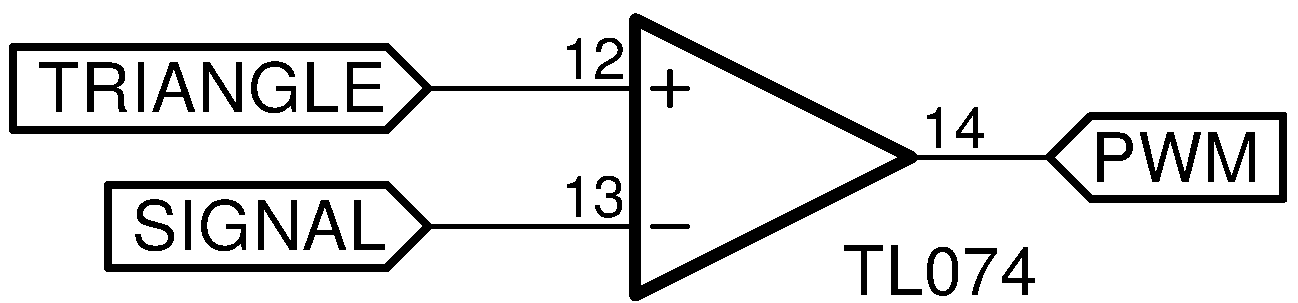
\includegraphics[width=6cm]{gfx/comp.pdf}
\caption{Komparator}
\label{fig:comp}
\end{floatingfigure}
\noindent
Der Komparator bildet das Kernstück zur Pulsweitenmodulation. Im wesentlichen vergleicht diese Komponente das im Dreiecksgenerator erzeugte Signal mit dem Eingangssignal und generiert damit die PWM (vgl. Abbildung \ref{fig:pwm}). Die Spezifikationen des für diese Aufgabe gewählten Operationsverstärkers sind von großer Bedeutung für die Funktionsfähigkeit und Skalierbarkeit des Gesamtsystems. Neben dem Stromverbrauch, der Betriebsspannung und der Slew-Rate ist auch die Beschaffbarkeit des Operationsvertärkers ein entscheidender Faktor. Für diese Anwendung wurde deswegen der TL074 gewählt, dieser zum einen durch die verwendete MOS-Technologie eine geringe Stromaufnahme von $< 14mA$ aufweist und zum Anderen mit einer Slew-Rate von $1V/ \mu s$ für diese Anwendung bestens geeignet ist.
\\
